\chapter{Zustände, Messungen und komplexe Vektorräume}

\lectureoverview{Die Quantenmechanik verändert zunächst, was wir unter einem Zustand verstehen. Zuerst isolieren wir das klassische Muster aus Zuständen und deterministischer Zustandsentwicklung; dann zeigt ein Spinexperiment mit zwei möglichen Ergebnissen, wo dieses Muster versagt. Die mathematische Antwort ist ein komplexer Vektorraum mit dualen Vektoren, einem Skalarprodukt, einer Norm und Orthogonalität.}

\section{Das klassische Muster: Zustand und Zustandsentwicklung}

Betrachten wir zunächst ein abgeschlossenes System, das zumindest vorübergehend von allem anderen isoliert ist. Das Wort \emph{System} ist hier ein Grundbegriff: Es bezeichnet das Objekt, dessen Geschichte wir vorhersagen wollen. Ein \emph{Zustand} umfasst alles, was wir zu einem bestimmten Zeitpunkt wissen müssen, um diese Vorhersage zu treffen. Die klassische Mechanik liefert ein Gesetz, das einen Zustand in den nächsten überführt.

Für die einfachste abstrakte Münze gilt
\begin{equation}
  \mathcal S_{\mathrm{coin}}=\{H,T\}.
\end{equation}
Ein mögliches Gesetz besagt, dass nichts geschieht:
\begin{equation}
  H\longmapsto H,
  \qquad
  T\longmapsto T.
\end{equation}
Ein anderes Gesetz lässt die beiden Zustände abwechseln:
\begin{equation}
  H\longmapsto T,
  \qquad
  T\longmapsto H.
\end{equation}
Diese Beispiele sind elementar, machen aber den Aufbau einer klassischen Theorie deutlich:
\begin{equation}
  s(t)\longmapsto s(t+\Delta t).
\end{equation}
Ist \(s(t)\) bekannt, so ist die Zustandsentwicklung deterministisch.

Dasselbe Muster gilt auch für kontinuierliche Zustandsräume. Für ein Teilchen, das sich auf einer Geraden bewegt, benötigt man sowohl seinen Ort als auch seinen Impuls,
\begin{equation}
  s=(q,p),
\end{equation}
sodass sein Zustandsraum die Phasenebene ist. Die Zahl möglicher Zustände ist nun unendlich, und die Gleichungen lassen sich in der eleganten Sprache der Lagrange-Funktionen, Hamilton-Funktionen und Poisson-Klammern formulieren. Die Grundidee bleibt jedoch dieselbe: Der Zustand zu einem Zeitpunkt enthält alles, was benötigt wird, um den Zustand zu einem anderen Zeitpunkt vorherzusagen.

\section{Abstraktion vor Anschauung}

Klassische Bewegung lässt sich vergleichsweise leicht veranschaulichen, weil ihre Begriffe der Alltagserfahrung entstammen. Dieser Vorteil geht verloren, wenn die betrachteten Objekte zu klein, die Geschwindigkeiten zu groß oder die Zustandsräume zu hochdimensional sind. Niemand kann sich die Bewegung eines Elektrons, die vierdimensionale Raumzeit oder einen zehn-dimensionalen Raum im wörtlichen Sinn vorstellen. Das ist keine besondere Schwäche von Anfängern. Die menschliche Anschauung ist auf die alltägliche dreidimensionale Welt zugeschnitten.

Selbst scheinbar einfachere Fälle zeigen diese Grenze. Was wir als Bild eines zweidimensionalen gekrümmten Raums bezeichnen, ist gewöhnlich eine Fläche, die in den dreidimensionalen Raum eingebettet ist. Eine eindimensionale Linie stellen wir uns als Strich in einer Ebene vor. Das Bild setzt stillschweigend den umgebenden Raum voraus, in dem sich unser Sehsystem orientieren kann.

Die Lösung besteht nicht darin, der ungewohnten Physik ein klassisches Bild aufzuzwingen. Vielmehr muss man die abstrakte Struktur erlernen und eine neue Anschauung aus korrekten Umformungen entwickeln. Aus dreidimensionalen Koordinaten \((x,y,z)\) werden vierdimensionale Koordinaten \((x,y,z,w)\), indem man ein Symbol hinzufügt und die Regeln erweitert, nicht indem man ein neues Sehorgan erhält. Die Quantenmechanik verlangt dieselbe Disziplin. Wer sie als ein seltsames mechanisches Modell kleiner klassischer Objekte behandelt, wird immer wieder zu falschen Ergebnissen gelangen.

\begin{remark}
Auch mathematische Anschauung entwickelt sich. Sie ist nur nicht dasselbe wie das Bild einer Meereswelle oder eines Pfeils im gewöhnlichen Raum. Die Algebra wird vertraut, wenn man ihre Beziehungen konsequent anwendet.
\end{remark}

\section{Klassische Zustandsräume und klassische Logik}

Für ein klassisches System ist der Zustandsraum eine Menge. Ein abstrakter Würfel hat
\begin{equation}
  \mathcal S_{\mathrm{die}}=\{1,2,3,4,5,6\}.
\end{equation}
Ein realer Würfel kann kontinuierlich viele Orientierungen einnehmen; der hier verwendete idealisierte Würfel besitzt jedoch nur diese sechs Bezeichnungen. Ein Teilchen auf einer Geraden hat die kontinuierlich unendliche Menge
\begin{equation}
  \mathcal S_{\mathrm{particle}}
  =
  \{(q,p)\mid q,p\in\mathbb R\}.
\end{equation}
Ob endlich oder unendlich: Jeder klassische Zustandsraum ist eine Sammlung voneinander verschiedener Möglichkeiten.

Eine Aussage über das System wählt eine Teilmenge dieser Möglichkeiten aus. Für den Würfel sei
\begin{align}
  P_{\mathrm{odd}}&=\{1,3,5\},\\
  P_{\leq 3}&=\{1,2,3\}.
\end{align}
Die Aussage \emph{ungerade und höchstens drei} entspricht dem Schnitt der beiden Mengen:
\begin{equation}
  P_{\mathrm{odd}}\cap P_{\leq 3}=\{1,3\}.
\end{equation}
Die inklusive Aussage \emph{ungerade oder höchstens drei} entspricht ihrer Vereinigung:
\begin{equation}
  P_{\mathrm{odd}}\cup P_{\leq 3}
  =
  \{1,2,3,5\}.
\end{equation}
Damit haben die klassische Konjunktion und Disjunktion mengentheoretisch die Form
\begin{equation}
  P\wedge Q\longleftrightarrow P\cap Q,
  \qquad
  P\vee Q\longleftrightarrow P\cup Q.
\end{equation}
Überlappen sich die Teilmengen nicht, gibt es keinen Zustand, in dem beide Aussagen wahr sind.

Diese Logik ist an das klassische Zustandskonzept gebunden. Die Quantenmechanik ersetzt die Menge klassischer Alternativen durch ein anderes mathematisches Objekt: einen Vektorraum. Erst im geeigneten klassischen Grenzfall verhält sich die Beschreibung durch einen Vektorraum näherungsweise wie eine Menge ausschließlicher Konfigurationen. Bevor wir diesen Raum konstruieren, brauchen wir ein Experiment, das den Ersatz unausweichlich macht.

\section{Das einfachste Quantensystem}

Das quantenmechanische Gegenstück zur abstrakten Münze ist ein System mit zwei möglichen Ergebnissen, ein sogenanntes \emph{Qubit}. Die gemessenen Alternativen lassen sich zunächst mit Kopf und Zahl bezeichnen; eine numerische Bezeichnung ist jedoch nützlicher:
\begin{equation}
  \sigma\in\{+1,-1\}.
\end{equation}
Wir verwenden parallel drei Schreibweisen:
\begin{equation}
  H\longleftrightarrow \sigma=+1\longleftrightarrow\uparrow,
  \qquad
  T\longleftrightarrow \sigma=-1\longleftrightarrow\downarrow.
\end{equation}
Zunächst sind die Pfeile lediglich Bezeichnungen. Ein gewöhnlicher geometrischer Vektor ist damit noch nicht vorausgesetzt.

\begin{figure}[htbp]
  \centering
  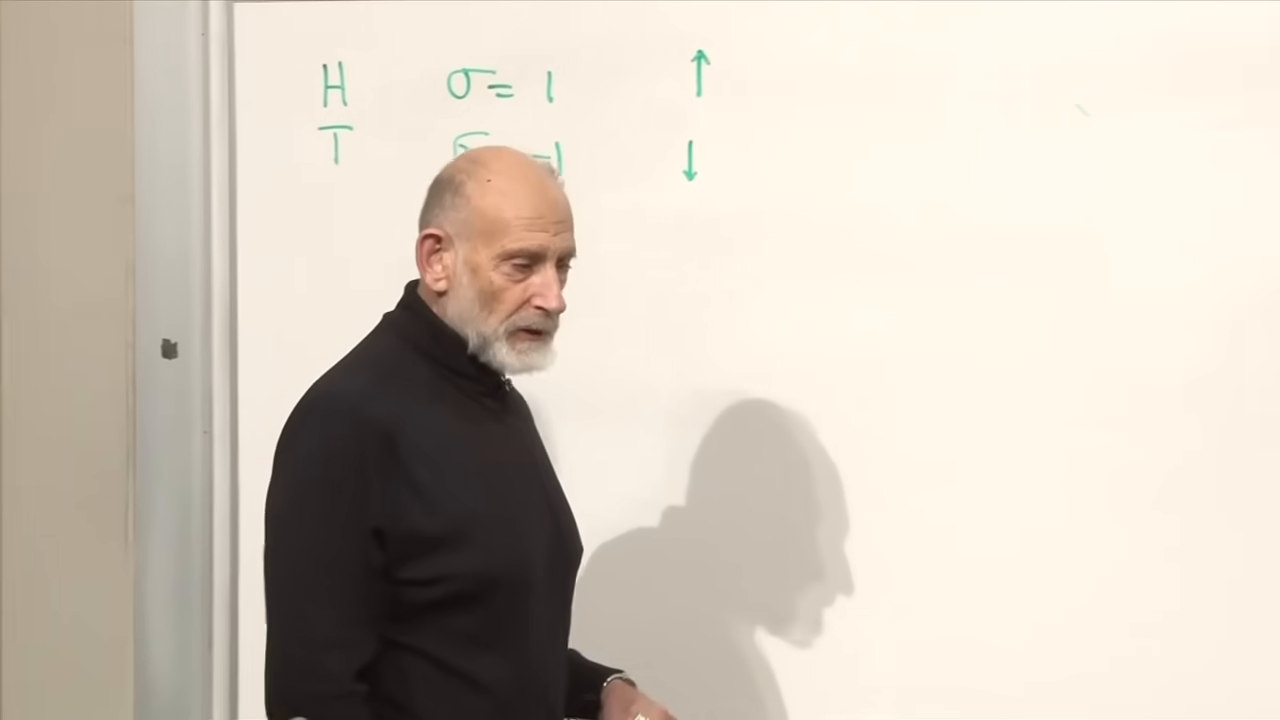
\includegraphics[width=0.78\textwidth]{lecture_01_figure_02.png}
  \caption{Die Tafel führt die gleichwertigen Bezeichnungen \(H/T\), \(\sigma=\pm1\) und die Pfeile für oben und unten ein. Die Pfeile sind zunächst Notation und kein klassisches Modell.}
  \lectureframe{00:22:44}
\end{figure}

\begin{classroomqa}
\audiencequestion{Was haben Kopf und Zahl mit dem physikalischen System zu tun?}
\lecturerresponse{Nichts, außer dass sie zwei vertraute Bezeichnungen liefern. Bei dieser Messung hat das Qubit zwei mögliche Ergebnisse; Kopf und Zahl sind Platzhalter. Die Bezeichnungen \(\pm1\) wurden gewählt, weil sie sich in Gleichungen verwenden lassen.}
\end{classroomqa}

\subsection{Der Apparat als Blackbox}

Für das Experiment benötigen wir ein zweites System, den Apparat \(A\). Vorerst ist er eine abstrakte Blackbox mit drei Eigenschaften:
\begin{enumerate}
  \item Er hat eine räumliche Orientierung, gekennzeichnet durch \emph{diese Seite oben};
  \item er besitzt einen Sensor, der mit dem Qubit wechselwirken kann;
  \item er hat eine Anzeige, die zunächst leer ist und anschließend \(+1\) oder \(-1\) anzeigt.
\end{enumerate}
Die Einzelheiten des Detektors lassen wir vorerst bewusst offen. Ein guter Detektor ist operational durch die zuverlässige Beziehung zwischen dem System und seiner Aufzeichnung definiert. Die beobachtende Person muss die Wechselwirkung nicht unmittelbar verfolgen; der Apparat kann das Ergebnis aufzeichnen, das später abgelesen wird.

Angenommen, die Anzeige meldet \(+1\). Setzen Sie den Apparat auf den leeren Zustand zurück und wiederholen Sie dieselbe Messung unmittelbar, bevor irgendeine unabhängige Entwicklung einsetzen kann. Ein zuverlässiger Detektor meldet erneut \(+1\). Lautet das erste Ergebnis \(-1\), so liefern unmittelbare Wiederholungen ebenfalls weiterhin \(-1\):
\begin{equation}
\begin{aligned}
  +1&\longrightarrow +1\longrightarrow +1\longrightarrow\cdots,\\
  -1&\longrightarrow -1\longrightarrow -1\longrightarrow\cdots.
\end{aligned}
\end{equation}
Die erste Messung kann daher als \emph{Präparation} aufgefasst werden. Sie versetzt das Qubit in einen Zustand, in dem eine unmittelbare Wiederholung derselben Messung ein eindeutiges Ergebnis liefert.

Diese Reproduzierbarkeit ist kein optionaler philosophischer Zusatz. Ohne sie gäbe es keine operationale Möglichkeit, eine Messung zu bestätigen. Ein defektes Gerät kann sein Ergebnis bei der Wiederholung verfehlen; dann führt es jedoch nicht die hier definierte ideale Messung aus.

\begin{classroomqa}
\audiencequestion{Ist das bereits der Kollaps der Wellenfunktion?}
\lecturerresponse{Diese Ausdrucksweise können wir später einführen. Vorerst genügt die operationale Aussage: Eine Messung liefert ein Ergebnis und präpariert einen Zustand, in dem dieselbe unmittelbare Messung dieses Ergebnis reproduziert. Den Vorgang zu benennen, erklärt ihn noch nicht.}
\end{classroomqa}

\section{Orientierung und das Scheitern des klassischen Zeigers}

Präparieren Sie das Qubit so, dass der aufrecht stehende Apparat \(+1\) anzeigt. Drehen Sie den Apparat um \(180^\circ\) und wiederholen Sie die Messung. Nun lautet das Ergebnis \(-1\). Wiederholte Messungen mit dem umgedrehten Apparat bestätigen \(-1\); wird der Apparat wieder aufgerichtet, ergibt sich erneut \(+1\).

Das Ergebnis zeigt eine echte Richtungsabhängigkeit. Die Notation für oben und unten ist nicht völlig willkürlich: Wird der Detektor umgedreht, kehrt sich das Vorzeichen um. Es liegt nahe, daraus zu schließen, das Qubit sei einfach ein kleiner Vektor und der Detektor messe die Komponente dieses Vektors entlang seiner eigenen Achse. Diese Vermutung muss jedoch geprüft und darf nicht einfach vorausgesetzt werden.

\begin{figure}[htbp]
  \centering
  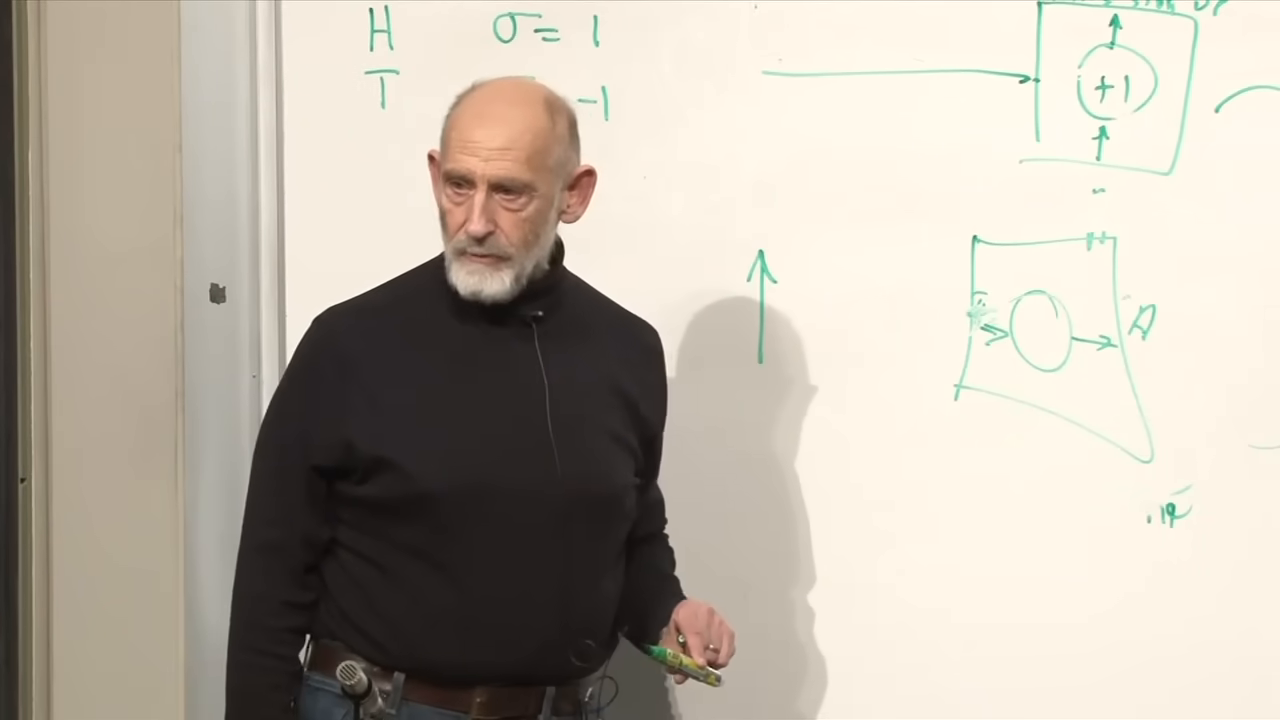
\includegraphics[width=0.82\textwidth]{lecture_01_figure_03.png}
  \caption{Eine Präparation mit Ergebnis nach oben und Analysatoren mit verschiedenen Orientierungen an der Tafel. Im weiteren Verlauf der Vorlesung wurde die Richtung eines Kreidepfeils korrigiert; für das Argument ist nur die Achse des Analysators entscheidend.}
  \lectureframe{00:36:21}
\end{figure}

\subsection{Eine Messung in Querrichtung}

Drehen Sie den Detektor um \(90^\circ\). Wäre das präparierte Qubit ein gewöhnlicher nach oben gerichteter Zeiger, wäre seine Komponente entlang der horizontalen Detektorachse null:
\begin{equation}
  \hat{\mathbf x}\cdot\hat{\mathbf z}=0.
\end{equation}
Der Quantenapparat zeigt niemals null an. Jeder einzelne Versuch liefert entweder \(+1\) oder \(-1\).

\begin{figure}[htbp]
  \centering
  \resizebox{\linewidth}{!}{%
  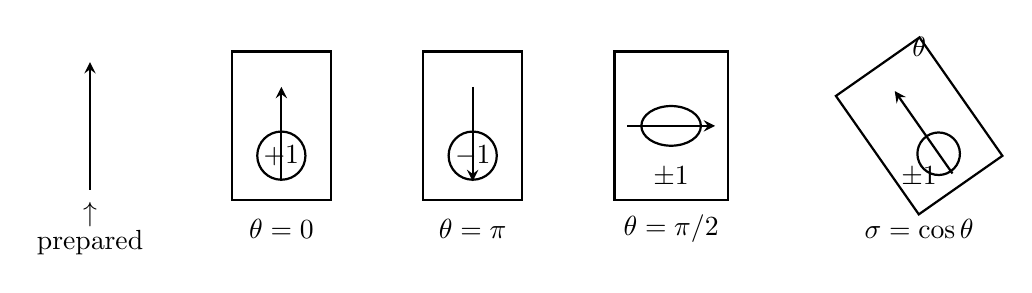
\begin{tikzpicture}[>=stealth,thick,scale=0.90]
    \draw[->] (0,0)--(0,1.8);
    \node at (0,-0.35) {\(\uparrow\)};
    \node at (0,-0.75) {prepared};

    \draw (2.0,-0.15) rectangle (3.4,1.95);
    \draw (2.7,0.48) circle (0.34);
    \draw[->] (2.7,0.12)--(2.7,1.45);
    \node at (2.7,0.48) {\(+1\)};
    \node at (2.7,-0.55) {\(\theta=0\)};

    \draw (4.7,-0.15) rectangle (6.1,1.95);
    \draw (5.4,0.48) circle (0.34);
    \draw[->] (5.4,1.45)--(5.4,0.12);
    \node at (5.4,0.48) {\(-1\)};
    \node at (5.4,-0.55) {\(\theta=\pi\)};

    \draw (7.4,-0.15) rectangle (9.0,1.95);
    \draw (8.2,0.90) ellipse (0.42 and 0.28);
    \draw[->] (7.58,0.90)--(8.82,0.90);
    \node at (8.2,0.18) {\(\pm1\)};
    \node at (8.2,-0.55) {\(\theta=\pi/2\)};

    \begin{scope}[shift={(11.7,0.90)},rotate=35]
      \draw (-0.72,-1.02) rectangle (0.72,1.02);
      \draw (0,-0.48) circle (0.30);
      \draw[->] (0,-0.82)--(0,0.60);
    \end{scope}
    \node at (11.7,0.18) {\(\pm1\)};
    \node at (11.7,-0.55) {\(\expect{\sigma}=\cos\theta\)};
    \node at (11.7,2.02) {\(\theta\)};
  \end{tikzpicture}
  }%
  \caption{Rekonstruktion der Analysatorfolge. Eine Drehung verändert die Statistik, niemals aber die Menge der möglichen Einzelergebnisse.}
\end{figure}

Präparieren Sie mit dem aufrecht stehenden Apparat eine große Anzahl von Qubits und behalten Sie diejenigen, bei denen das Ergebnis \(+1\) lautet. Messen Sie jedes dieser Qubits einmal mit dem seitlich ausgerichteten Apparat. Die Hälfte der Versuche ergibt \(+1\), die andere Hälfte \(-1\); der Ensemblemittelwert ist null:
\begin{equation}
  \expect{\sigma}_{\pi/2}=0.
\end{equation}
Der Mittelwert ähnelt der verschwindenden horizontalen Komponente eines klassischen Zeigers, die einzelnen Aufzeichnungen jedoch nicht. Der klassische Wert \(0\) ist durch ein statistisches Gleichgewicht zwischen zwei diskreten Ergebnissen ersetzt worden.

\begin{classroomqa}
\audiencequestion{Was geschieht, wenn man dasselbe Qubit nach der seitlichen Messung behält, statt es zu verwerfen?}
\lecturerresponse{Angenommen, das erste seitliche Messergebnis lautet \(+1\). Wiederholt man die seitliche Messung an diesem selben Qubit, erhält man immer wieder \(+1\). Die erste seitliche Messung hat das Qubit relativ zur seitlichen Achse präpariert. Um die Statistik mit gleichen Häufigkeiten zu erhalten, muss man das gesamte Präparations- und Messverfahren an vielen Qubits wiederholen, statt ein einzelnes Ergebnis wiederholt zu bestätigen.}
\end{classroomqa}

\subsection{Unvereinbare Präparationen}

Die Reihenfolge der Achsen ist entscheidend. Präparieren Sie \(+1\) in vertikaler Richtung und messen Sie anschließend horizontal. Das erste horizontale Messergebnis ist zufällig. Sobald ein horizontales Ergebnis vorliegt, sind unmittelbar folgende horizontale Wiederholungen eindeutig. Richten Sie den Detektor nun wieder vertikal aus. Das vertikale Ergebnis ist erneut zufällig.

Bezeichnen \(M_z\) und \(M_x\) Messungen entlang der beiden Achsen, so gilt in Symbolen:
\begin{equation}
\begin{aligned}
  M_z&:+1,\\
  M_x&:\pm1,\\
  M_x&:\text{same result},\\
  M_z&:\pm1.
\end{aligned}
\end{equation}
Die dazwischenliegende \(x\)-Messung hat nicht lediglich eine horizontale Komponente aufgedeckt und dabei den ursprünglichen vertikalen Zustand erhalten. Sie hat einen neuen Zustand präpariert; die ursprüngliche Eindeutigkeit bezüglich der vertikalen Achse ist verloren.

\begin{classroomqa}
\audiencequestion{Erinnert sich der Detektor an die erste Antwort? Woher weiß er, ob dasselbe oder ein neues Qubit vorgelegt wurde?}
\lecturerresponse{Die Reproduzierbarkeit ist eine Eigenschaft des gemessenen Qubits und beruht nicht darauf, dass der Detektor eine verborgene Erinnerung mit dem Ergebnis vergleicht. Nach einer Messung befindet sich das Qubit in einem Zustand, der bei derselben unmittelbaren Messung dasselbe Ergebnis liefert. Wird ein anders präpariertes Qubit vorgelegt, hängt das Ergebnis von dieser Präparation ab. Nachzuhalten, welches physikalische System gerade gemessen wird, gehört zur gewöhnlichen Laborpraxis.}
\end{classroomqa}

\begin{classroomqa}
\audiencequestion{Präpariert die Beobachtungshandlung also das jeweilige Qubit?}
\lecturerresponse{Ja. Sobald die Messung das Qubit präpariert hat, liefert dieselbe Messung weiterhin dasselbe Ergebnis, bis eine andere Entwicklung oder eine unvereinbare Messung dazwischenkommt.}
\end{classroomqa}

\section{Ein beliebig gedrehter Analysator}

Die Detektorachse bilde mit der Achse, entlang der das Ensemble präpariert wurde, einen Winkel \(\theta\). Jeder Versuch liefert weiterhin
\begin{equation}
  \sigma=\pm1.
\end{equation}
Die relativen Häufigkeiten ändern sich mit dem Winkel, sodass der Mittelwert
\begin{equation}
  \expect{\sigma}_{\theta}=\cos\theta.
  \label{eq:qml1-cosine-mean}
\end{equation}
beträgt. Die Grenzfälle sind
\begin{align}
  \expect{\sigma}_{0}&=+1,\\
  \expect{\sigma}_{\pi/2}&=0,\\
  \expect{\sigma}_{\pi}&=-1.
\end{align}
Für Winkel nahe \(\theta=0\) sind die meisten Ergebnisse \(+1\), gelegentlich tritt \(-1\) auf. Für Winkel nahe \(\theta=\pi\) sind die meisten Ergebnisse \(-1\), gelegentlich tritt \(+1\) auf.

\begin{figure}[htbp]
  \centering
  \includegraphics[width=0.82\textwidth]{lecture_01_figure_04.png}
  \caption{Die tatsächliche Tafelzeichnung zum Experiment mit beliebigem Winkel: Ein vertikal präpariertes Ensemble trifft auf einen um \(\theta\) geneigten Analysator.}
  \lectureframe{00:48:55}
\end{figure}

Die Größe, die sich wie ein glatter Vektor verhält, ist der Ensemblemittelwert, nicht das Einzelergebnis. Sind \(p_+(\theta)\) und \(p_-(\theta)\) die beiden Wahrscheinlichkeiten, so gilt
\begin{equation}
  p_+ + p_-=1,
  \qquad
  p_+-p_-=\cos\theta.
\end{equation}
Folglich ist
\begin{equation}
\begin{aligned}
  p_+(\theta)&=\frac{1+\cos\theta}{2}
  =\cos^2\frac{\theta}{2},\\
  p_-(\theta)&=\frac{1-\cos\theta}{2}
  =\sin^2\frac{\theta}{2}.
\end{aligned}
  \label{eq:qml1-half-angle-probabilities}
\end{equation}
\editorialnote{In der Vorlesung werden die beiden Ergebnisse und ihr Mittelwert \(\cos\theta\) angegeben. Gleichung~\eqref{eq:qml1-half-angle-probabilities} folgt unmittelbar algebraisch aus diesen Aussagen und macht das implizite Häufigkeitsgesetz explizit.}

\begin{classroomqa}
\audiencequestion{Zeigt auch ein unpräpariertes Qubit-Ensemble den Mittelwert \(\cos\theta\)?}
\lecturerresponse{In einem unpolarisierten Ensemble ist keine bestimmte Richtung ausgewählt, daher ist sein Mittelwert null. Die Abhängigkeit von \(\theta\) bezieht sich auf ein Ensemble, das zuvor entlang einer bestimmten Achse präpariert wurde.}
\end{classroomqa}

\begin{classroomqa}
\audiencequestion{Warum braucht man ein ganzes Ensemble, wenn sich das Qubit dazwischen nicht weiterentwickelt?}
\lecturerresponse{Die erste Messung an einem einzelnen Qubit mit geneigtem Analysator liefert eine Stichprobe. Jede unmittelbare Wiederholung an demselben Qubit bestätigt lediglich dieses Ergebnis. Unabhängige Versuche erfordern identisch präparierte Qubits, die jeweils einmal mit dem geneigten Analysator gemessen werden.}
\end{classroomqa}

\begin{classroomqa}
\audiencequestion{Gibt es Muster oder Korrelationen höherer Ordnung in der Folge der Plus- und Minuszeichen?}
\lecturerresponse{Für dieses Experiment nehmen wir an, dass die einzelnen Versuche unabhängig und unkorreliert sind. Ihre Einzelversuchswahrscheinlichkeiten hängen von \(\theta\) ab; ein zusätzliches Ordnungsmuster wird jedoch nicht behauptet.}
\end{classroomqa}

\subsection{Was idealisiert wurde}

Vorerst behandeln wir den Apparat als klassisches Objekt mit kontinuierlich einstellbarer Orientierung und diskreter Anzeige. Diese Trennung zwischen \emph{System} und \emph{Detektor} ist vorläufig. Auch der Detektor ist ein physikalisches System und muss letztlich der Quantenmechanik gehorchen. Eine vollständige Beschreibung muss System und Apparat gemeinsam behandeln; dafür fehlen uns bislang jedoch die nötigen Mittel.

\begin{classroomqa}
\audiencequestion{Ist der Detektor selbst einfach ein weiteres Zweizustandssystem?}
\lecturerresponse{Er besitzt physikalische Zustände und muss letztlich in die quantenmechanische Beschreibung aufgenommen werden. Vorerst behalten wir eine operationale Trennung bei: Das Qubit ist das Objekt, das quantenmechanisch beschrieben wird, während der orientierte Detektor eine stabile klassische Aufzeichnung liefert. Später muss das Gesamtsystem als Wechselwirkung quantenmechanischer Systeme analysiert werden.}
\end{classroomqa}

\begin{classroomqa}
\audiencequestion{Führt die Änderung der Achse, um die der Detektor gedreht wird, zu einer reichhaltigeren Struktur als dem hier gezeigten einzelnen Winkel?}
\lecturerresponse{Ja, die vollständige dreidimensionale Beschreibung ist umfangreicher. Die Drehung in einer Ebene ist ihr einfachster Ausschnitt und stimmt mit der später folgenden umfassenderen Behandlung überein.}
\end{classroomqa}

\begin{classroomqa}
\audiencequestion{Kann der Detektor einen kontinuierlichen Wert zwischen \(-1\) und \(+1\) anzeigen?}
\lecturerresponse{Seine Orientierung lässt sich kontinuierlich verändern, doch jede ideale Qubitmessung liefert weiterhin \(+1\) oder \(-1\). Kontinuität tritt bei veränderter Orientierung in den Wahrscheinlichkeiten und Mittelwerten auf, nicht in den Einzelergebnissen.}
\end{classroomqa}

\section{Zeiger und abstrakte Vektoren}

Die experimentellen Tatsachen stellen wir nun eine Weile zurück und wenden uns der Mathematik zu. Ein gewöhnlicher Pfeil im physikalischen Raum soll \emph{Zeiger} heißen. Ein mathematischer Vektor ist allgemeiner: Er ist ein Element eines Vektorraums und muss nicht in eine Richtung im gewöhnlichen Raum zeigen.

\begin{definition}Ein komplexer Vektorraum \(V\) ist eine Menge von Vektoren, für die Vektoraddition und Multiplikation mit komplexen Skalaren definiert sind und die üblichen Linearitätsregeln erfüllen. Insbesondere gilt für \(u,v,w\in V\) und \(a,b\in\mathbb C\):
\begin{align}
  u+v&=v+u,\\
  (u+v)+w&=u+(v+w),\\
  a(u+v)&=au+av,\\
  (a+b)u&=au+bu,\\
  (ab)u&=a(bu),\\
  1u&=u.
\end{align}
Es gibt einen Nullvektor \(0\) und zu jedem \(u\) einen additiv inversen Vektor \(-u\).
\end{definition}

In der Diskussion an der Tafel werden zunächst nur die Operationen und die Abgeschlossenheit betont:
\begin{equation}
\begin{aligned}
  u,v\in V&\Longrightarrow u+v\in V,\\
  a\in\mathbb C,\ u\in V&\Longrightarrow au\in V.
\end{aligned}
\end{equation}
Der Nullvektor und die Kommutativität werden anschließend als Antwort auf Fragen ergänzt. Die übrigen vertrauten Axiome führen ausdrücklich auf, was bei der Einführung des konkreten Modells mit Spaltenvektoren ohnehin bereits verwendet wird.

Die reellen Zahlen bilden einen eindimensionalen Vektorraum über \(\mathbb R\). Die komplexen Zahlen bilden einen eindimensionalen Vektorraum über \(\mathbb C\) und einen zweidimensionalen Vektorraum über \(\mathbb R\). Auch komplexwertige Funktionen \(\psi(x)\) bilden einen komplexen Vektorraum, denn
\begin{equation}
  (\psi+\phi)(x)=\psi(x)+\phi(x),
  \qquad
  (z\psi)(x)=z\psi(x).
\end{equation}
Dieses Beispiel eines Funktionenraums wird später zentral sein; zunächst lässt sich die Struktur jedoch an endlichdimensionalen Spalten leichter erkennen.

\begin{classroomqa}
\audiencequestion{Worin besteht der Unterschied zwischen einem Vektor und einem Vektorraum?}
\lecturerresponse{Ein Vektor ist ein einzelnes Element. Ein Vektorraum ist die Menge all dieser Elemente zusammen mit den Regeln für ihre Addition und Multiplikation mit Skalaren. Das ist vergleichbar mit einer einzelnen Zahl und dem Zahlensystem, das eine Menge von Zahlen samt Operationen umfasst.}
\end{classroomqa}

\section{Komplexe Spalten mit zwei Komponenten}

Schreiben wir einen abstrakten Vektor in Dirac-Notation als \(\ket{\alpha}\). Eine konkrete Darstellung ist
\begin{equation}
  \ket{\alpha}
  \longleftrightarrow
  \begin{pmatrix}
    \alpha_1\\
    \alpha_2
  \end{pmatrix},
  \qquad
  \alpha_1,\alpha_2\in\mathbb C.
\end{equation}
Gilt
\begin{equation}
  \ket{\beta}
  \longleftrightarrow
  \begin{pmatrix}
    \beta_1\\
    \beta_2
  \end{pmatrix},
\end{equation}
so sind Addition und Skalarmultiplikation komponentenweise definiert:
\begin{align}
  \ket{\alpha}+\ket{\beta}
  &\longleftrightarrow
  \begin{pmatrix}
    \alpha_1+\beta_1\\
    \alpha_2+\beta_2
  \end{pmatrix},\\
  z\ket{\alpha}
  &\longleftrightarrow
  \begin{pmatrix}
    z\alpha_1\\
    z\alpha_2
  \end{pmatrix},
  \qquad z\in\mathbb C.
\end{align}

\begin{figure}[htbp]
  \centering
  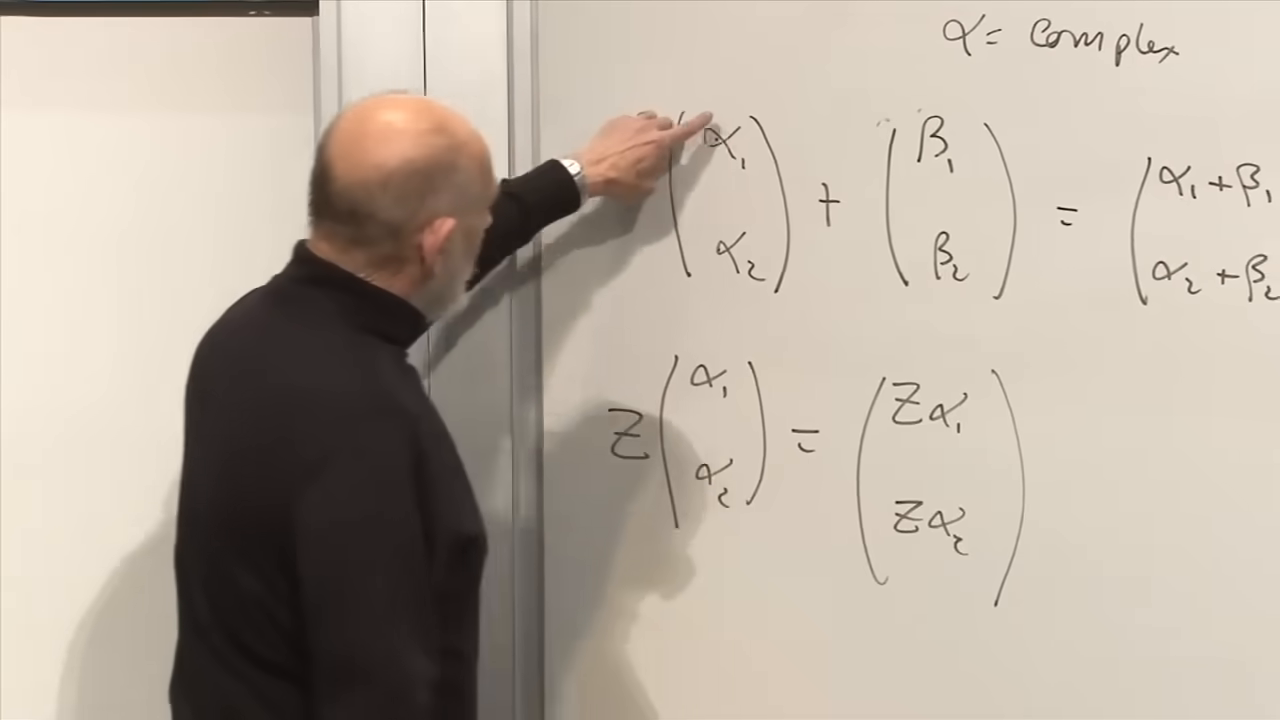
\includegraphics[width=0.88\textwidth]{lecture_01_figure_05.png}
  \caption{Die komponentenweisen Regeln für die Addition zweier komplexer Spalten und die Multiplikation einer Spalte mit einem komplexen Skalar.}
  \lectureframe{01:14:28}
\end{figure}

Der Nullvektor ist
\begin{equation}
  \ket{0}
  =
  \begin{pmatrix}
    0\\
    0
  \end{pmatrix},
  \qquad
  \ket{\alpha}+\ket{0}=\ket{\alpha}.
\end{equation}
Spalten der Länge drei bilden einen weiteren Vektorraum; dasselbe gilt für jede fest gewählte Länge. Eine Spalte mit zwei Komponenten lässt sich nicht zu einer Spalte mit drei Komponenten addieren, da beide zu verschiedenen Räumen gehören und keine komponentenweise Regel sie miteinander verknüpft.

\begin{classroomqa}
\audiencequestion{Ist ein Spaltenvektor eine Matrix?}
\lecturerresponse{In der allgemeinen Terminologie ist er eine Matrix mit einer Spalte. In dieser Vorlesung bezeichnet das Wort \emph{Matrix} gewöhnlich eine quadratische Anordnung; eine Anordnung mit nur einer Spalte nennen wir Spaltenvektor. Der Unterschied ist terminologischer Art und bedeutet keine unterschiedliche Auffassung der Algebra.}
\end{classroomqa}

\begin{classroomqa}
\audiencequestion{Spielt die Reihenfolge bei der Vektoraddition eine Rolle?}
\lecturerresponse{Nein. Die komponentenweise Addition übernimmt die Kommutativität der komplexen Zahlen:
\[
  \ket{\alpha}+\ket{\beta}
  =
  \ket{\beta}+\ket{\alpha}.
\]
Dies ist eines der Vektorraumaxiome.}
\end{classroomqa}

\section{Dualvektoren: Bras und Kets}

Zu jedem Ket \(\ket{A}\) gehört ein entsprechender Vektor im Dualraum, geschrieben als \(\bra{A}\). Die Abbildung vom Ket zum Bra ist additiv, konjugiert aber komplexe Skalare:
\begin{align}
  \ket{A}+\ket{B}
  &\longleftrightarrow
  \bra{A}+\bra{B},\\
  z\ket{A}
  &\longleftrightarrow
  z^*\bra{A}.
  \label{eq:qml1-antilinear-dual}
\end{align}
Diese zweite Regel ist das entscheidende Merkmal im komplexen Fall. Das Dual eines skalarvielfachen Vektors wird mit dem komplex konjugierten Skalar multipliziert.

\begin{figure}[htbp]
  \centering
  \includegraphics[width=0.86\textwidth]{lecture_01_figure_06.png}
  \caption{Die Zuordnung vom Ket zum Bra und ihre beiden Regeln: Summen werden auf Summen abgebildet, bei der Skalarmultiplikation wird hingegen komplex konjugiert.}
  \lectureframe{01:23:15}
\end{figure}

Für die Darstellung mit zwei Komponenten gilt
\begin{equation}
  \ket{\alpha}
  =
  \begin{pmatrix}
    \alpha_1\\
    \alpha_2
  \end{pmatrix}
  \qquad\Longrightarrow\qquad
  \bra{\alpha}
  =
  \begin{pmatrix}
    \alpha_1^*&\alpha_2^*
  \end{pmatrix}.
  \label{eq:qml1-bra-from-ket}
\end{equation}
Die komplexe Konjugation realisiert die Dualzuordnung, und die Zeilenschreibweise macht die beiden Arten von Objekten sichtbar unterscheidbar. Gleichung~\eqref{eq:qml1-bra-from-ket} bestätigt außerdem Gleichung~\eqref{eq:qml1-antilinear-dual} unmittelbar.

\section{Das Skalarprodukt}

Für \(\ket{\alpha}\) und \(\ket{\beta}\) bilden wir aus dem zu \(\beta\) gehörenden Bra und dem Ket \(\alpha\) das Skalarprodukt:
\begin{equation}
  \braket{\beta}{\alpha}
  =
  \begin{pmatrix}
    \beta_1^*&\beta_2^*
  \end{pmatrix}
  \begin{pmatrix}
    \alpha_1\\
    \alpha_2
  \end{pmatrix}
  =
  \beta_1^*\alpha_1+\beta_2^*\alpha_2.
  \label{eq:qml1-inner-product}
\end{equation}
Das Wort \emph{Klammerausdruck} setzt sich wörtlich aus \emph{Bra} und \emph{Ket} zusammen. Es handelt sich um das komplexe Analogon des Skalarprodukts: Man multipliziert die entsprechenden Komponenten und addiert sie; dabei werden die Komponenten des Bras komplex konjugiert.

\begin{figure}[htbp]
  \centering
  \includegraphics[width=0.88\textwidth]{lecture_01_figure_07.png}
  \caption{An der Tafel wird das Skalarprodukt \(\braket{\beta}{\alpha}\) zu \(\beta_1^*\alpha_1+\beta_2^*\alpha_2\) berechnet.}
  \lectureframe{01:31:25}
\end{figure}

Vertauscht man die Vektoren, erhält man
\begin{equation}
  \braket{\alpha}{\beta}
  =
  \alpha_1^*\beta_1+\alpha_2^*\beta_2
  =
  \braket{\beta}{\alpha}^{*}.
  \label{eq:qml1-conjugate-symmetry}
\end{equation}
Die Reihenfolge spielt also im Allgemeinen eine Rolle, allerdings nur insofern, als sich das Ergebnis komplex konjugiert.

\begin{classroomqa}
\audiencequestion{Könnte man ein Produkt komplexer Vektoren ohne Konjugation einer Seite definieren?}
\lecturerresponse{Man kann einen solchen bilinearen Ausdruck definieren; dann muss das Produkt eines Vektors mit sich selbst jedoch weder reell noch positiv sein. Für die Quantenmechanik ist diese Struktur nicht zweckmäßig. Das konjugierte, also hermitesche Skalarprodukt liefert die Norm und die Wahrscheinlichkeitsstruktur, die wir benötigen werden.}
\end{classroomqa}

\subsection{Norm und Positivität}

Setzen wir \(\beta=\alpha\) in Gleichung~\eqref{eq:qml1-inner-product} ein:
\begin{equation}
  \braket{\alpha}{\alpha}
  =
  \alpha_1^*\alpha_1+\alpha_2^*\alpha_2
  =
  |\alpha_1|^2+|\alpha_2|^2.
  \label{eq:qml1-norm-square}
\end{equation}
Diese Zahl ist gleich ihrer eigenen komplexen Konjugierten und daher reell. Sie ist nichtnegativ und verschwindet nur beim Nullvektor. Die Länge ist definiert durch
\begin{equation}
  \|\alpha\|
  =
  \sqrt{\braket{\alpha}{\alpha}}.
\end{equation}
Komplexe Komponenten ergeben somit eine gewöhnliche, nichtnegative reelle Länge.

\begin{figure}[htbp]
  \centering
  \includegraphics[width=0.88\textwidth]{lecture_01_figure_08.png}
  \caption{Das Selbstskalarprodukt an der Tafel: \(\braket{\alpha}{\alpha}=|\alpha_1|^2+|\alpha_2|^2\), das Quadrat der Norm.}
  \lectureframe{01:34:40}
\end{figure}

\section{Orthogonalität und Dimension}

Zwei Vektoren heißen orthogonal, wenn ihr Skalarprodukt verschwindet:
\begin{equation}
  \braket{\beta}{\alpha}=0.
  \label{eq:qml1-orthogonality}
\end{equation}
Dank der konjugierten Symmetrie ist diese Beziehung unabhängig von der Reihenfolge:
\begin{equation}
  \braket{\beta}{\alpha}=0
  \quad\Longrightarrow\quad
  \braket{\alpha}{\beta}
  =
  \braket{\beta}{\alpha}^{*}
  =0.
\end{equation}

Im Raum mit zwei Komponenten ist das einfachste orthogonale Paar
\begin{equation}
  \ket{e_1}
  =
  \begin{pmatrix}
    1\\
    0
  \end{pmatrix},
  \qquad
  \ket{e_2}
  =
  \begin{pmatrix}
    0\\
    1
  \end{pmatrix},
  \qquad
  \braket{e_1}{e_2}=0.
  \label{eq:qml1-standard-basis}
\end{equation}

\begin{figure}[htbp]
  \centering
  \includegraphics[width=0.88\textwidth]{lecture_01_figure_09.png}
  \caption{An der Tafel werden die Standardvektoren \((1,0)^{\mathsf T}\) und \((0,1)^{\mathsf T}\) als orthogonales Paar konstruiert.}
  \lectureframe{01:39:50}
\end{figure}

Die Dimension lässt sich als die größtmögliche Anzahl paarweise orthogonaler, von null verschiedener Vektoren charakterisieren. In einem zweidimensionalen Raum kann es zwei solche Vektoren geben, aber keinen dritten. Betrachten wir dazu konkret
\begin{equation}
  \ket{v}
  =
  \begin{pmatrix}
    v_1\\
    v_2
  \end{pmatrix}
\end{equation}
und nehmen an, dieser Vektor sei zu beiden Vektoren in Gleichung~\eqref{eq:qml1-standard-basis} orthogonal. Dann gilt
\begin{equation}
  \braket{e_1}{v}=v_1=0,
  \qquad
  \braket{e_2}{v}=v_2=0,
\end{equation}
also \(\ket{v}=\ket{0}\). Es gibt keinen dritten von null verschiedenen Vektor, der zu beiden orthogonal ist.

\begin{classroomqa}
\audiencequestion{Ist der Nullvektor nicht zu jedem Vektor orthogonal und damit ein zusätzlicher Vektor?}
\lecturerresponse{Ja. Deshalb muss die Definition von paarweise orthogonalen Vektoren ausdrücklich verlangen, dass sie \emph{von null verschieden} sind. Der Nullvektor trägt keine unabhängige Richtung bei und wird bei der Bestimmung der Dimension nicht mitgezählt.}
\end{classroomqa}

\begin{remark}In der Spaltendarstellung entspricht die Dimension der Anzahl der Komponenten. Die Definition über Orthogonalität ist abstrakter und setzt keine zuvor gewählten Koordinaten voraus.
\end{remark}

\section{Weitere Fragen an der Tafel}

\begin{classroomqa}
\audiencequestion{Gilt dieselbe Struktur auch für einen Funktionenvektorraum?}
\lecturerresponse{Ja. Eine Funktion lässt sich als Spalte mit einer kontinuierlich indizierten Familie von Einträgen \(\psi(x)\) auffassen. Addition und Skalarmultiplikation erfolgen punktweise. Das entsprechende Skalarprodukt wird statt einer endlichen Summe ein Integral sein; diese Konstruktion behandeln wir später.}
\end{classroomqa}

\begin{classroomqa}
\audiencequestion{Ergibt die Multiplikation eines Kets mit einem Bra eine Matrix?}
\lecturerresponse{Ja. Das Skalarprodukt \(\bra{\beta}\ket{\alpha}\) verknüpft eine Zeile mit einer Spalte und ergibt eine Zahl. Bei umgekehrter Reihenfolge, \(\ket{\alpha}\bra{\beta}\), erhält man ein äußeres Produkt, also eine quadratische Matrix. Sowohl innere als auch äußere Produkte werden wichtig sein.}
\end{classroomqa}

\begin{classroomqa}
\audiencequestion{Beeinflusst die Messung das Qubit tatsächlich, statt es lediglich zu enthüllen?}
\lecturerresponse{Ja. Die erste Messung entlang einer neuen Achse präpariert einen neuen Zustand. Deshalb bestätigt eine Wiederholung dieser Messung das Ergebnis, während die Rückkehr zur ursprünglichen Achse erneut Unbestimmtheit hervorruft. Diese unvermeidliche Störung unterscheidet das Quantenexperiment von einer idealisierten klassischen Messung, die sich prinzipiell beliebig schonend durchführen lässt.}
\end{classroomqa}

\section{Die beiden Hälften der Konstruktion}

Wir haben nun zwei Hälften, die bislang noch nicht miteinander verknüpft sind. Die experimentelle Hälfte besagt:
\begin{enumerate}
  \item Eine ideale Qubitmessung hat nur die Ergebnisse \(\pm1\);
  \item die Wiederholung derselben unmittelbaren Messung bestätigt das Ergebnis;
  \item eine Änderung der Detektorachse verändert den durch die Messung präparierten Zustand;
  \item für ein präpariertes Ensemble hat ein um \(\theta\) geneigter Analysator den Mittelwert \(\cos\theta\).
\end{enumerate}
Die mathematische Hälfte besagt:
\begin{enumerate}
  \item Quantenzustände werden durch Vektoren statt durch klassische Punkte dargestellt;
  \item die relevanten Vektoren bilden einen komplexen Vektorraum;
  \item zu Kets gehören duale Bras, die sich bei komplexer Skalierung antilinear verhalten;
  \item das hermitesche Skalarprodukt definiert Länge, Orthogonalität und Dimension.
\end{enumerate}

Die nächste Aufgabe besteht darin, diese beiden Hälften miteinander zu verknüpfen. Der zweidimensionale komplexe Zustandsraum eines Qubits muss die Wiederholbarkeit, Zufälligkeit und winkelabhängige Statistik des Analysatorexperiments reproduzieren. Diese Verbindung, nicht irgendein verborgenes klassisches Bild, ist der Ausgangspunkt der Quantenmechanik.
